\documentclass[12pt]{beamer}
\usepackage{helvet} %font
\beamertemplatenavigationsymbolsempty
%\usetheme{Rochester}
\usefonttheme{structurebold}

\usepackage[french]{babel}
\usepackage[utf8]{inputenc}
\usepackage[T1]{fontenc}
\usepackage{amssymb,amsmath,amsfonts,amsthm}
\usepackage{verbatim}
\usepackage{graphicx}
\usepackage{layout}
\usepackage{float}
\usepackage{tikz}
\usepackage{pgf}
\usepackage{cancel}
\usepackage{makeidx}
\usepackage{tabularx}
\usepackage{multirow}
\usepackage{enumitem}

%\setbeamercolor{structure}{fg=red}
\setbeamercolor{frametitle}{bg=white,fg=black}

\author{}
\date{}

\begin{document}

\begin{frame}
\begin{tabular}{b{7cm}l}
& \multirow{2}{*}{\includegraphics[scale=0.25]{samm.png}}\\ {\large \textbf{Collecte des Données (1/2)}}& 
\end{tabular}

\vspace{1.5cm}

\textbf{Problèmes :}\\

\vspace{0.5cm}
\setlist[itemize]{label=\textbullet}
\begin{itemize}
	\item Pas de corpus a priori
	\item Pas d'API
	\item Pas de structuration uniforme
	\item Pas d'encodage uniforme
	\item Pas d'unicité des références
\end{itemize}


\end{frame}

\begin{frame}
\begin{tabular}{b{7cm}l}
& \multirow{2}{*}{\includegraphics[scale=0.25]{samm.png}}\\ {\large \textbf{Collecte des Données (2/2)}}& 
\end{tabular}

\vspace{1.5cm}

\textbf{Démarche :}\\

\vspace{0.5cm}
\setlist[itemize]{label=\textbullet}
\begin{itemize}
	\item Identification arbitraire d'un corpus avec temps d'arrêt
	\item Extraction récursive des liens avec élagage
	\item Extraction des contenus
	\item Extraction des textes propres
	\item Décodage
	\item Stopwords et lemmatisation
\end{itemize}

\end{frame}

\begin{frame}
\begin{tabular}{b{7cm}l}
& \multirow{2}{*}{\includegraphics[scale=0.25]{samm.png}}\\ {\large \textbf{Exemple}}& 
\end{tabular}

\vspace{0.5cm}

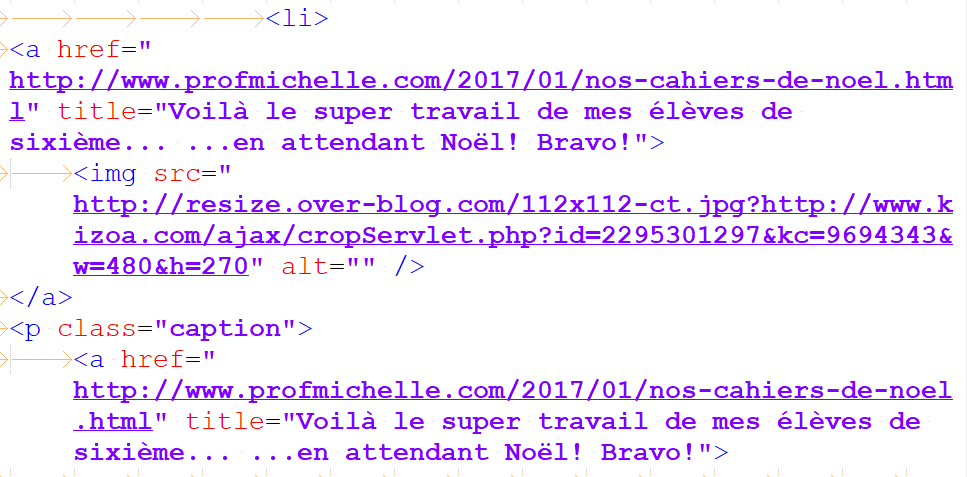
\includegraphics[scale=0.25]{code1-liens.png}

\end{frame}

\begin{frame}
\begin{tabular}{b{7cm}l}
& \multirow{2}{*}{\includegraphics[scale=0.25]{samm.png}}\\ {\large \textbf{Exemple}}& 
\end{tabular}

\vspace{0.5cm}

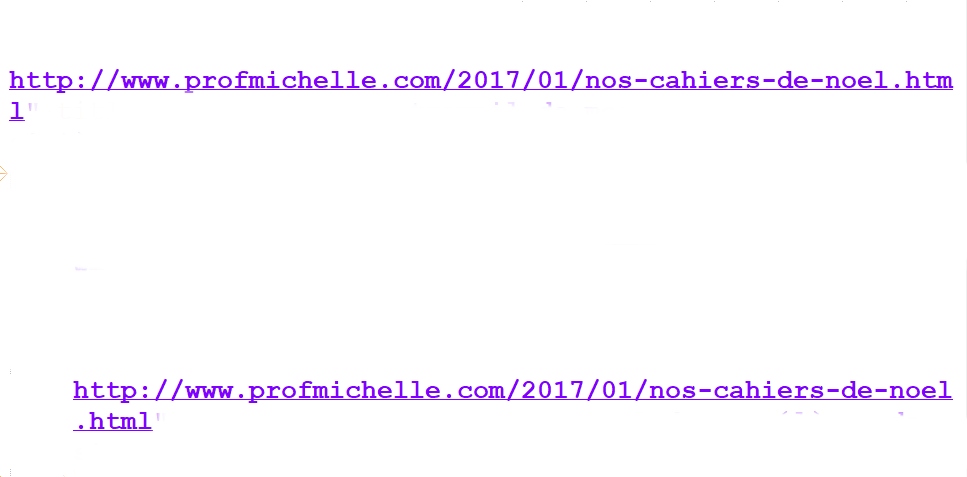
\includegraphics[scale=0.25]{code1-liens2.png}

\end{frame}

\begin{frame}
\begin{tabular}{b{7cm}l}
& \multirow{2}{*}{\includegraphics[scale=0.25]{samm.png}}\\ {\large \textbf{Exemple}}& 
\end{tabular}

\vspace{0.5cm}

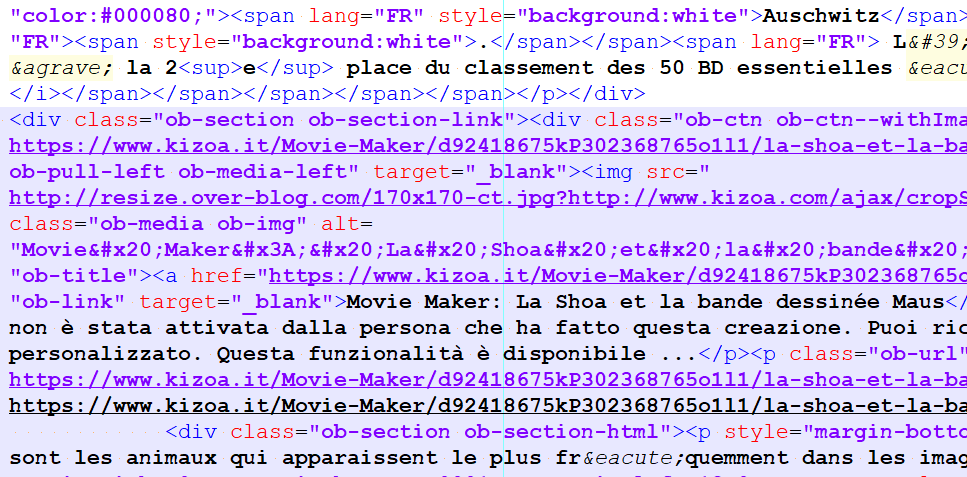
\includegraphics[scale=0.25]{code2-brut.png}

\end{frame}

\begin{frame}
\begin{tabular}{b{7cm}l}
& \multirow{2}{*}{\includegraphics[scale=0.25]{samm.png}}\\ {\large \textbf{Exemple}}& 
\end{tabular}

\vspace{0.5cm}

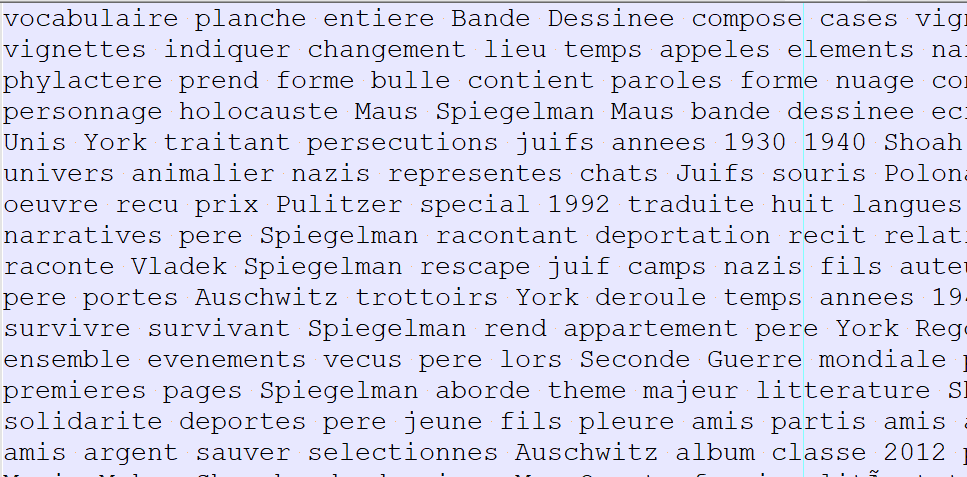
\includegraphics[scale=0.25]{code3-sac.png}

\end{frame}

\begin{frame}
\begin{tabular}{b{7cm}l}
& \multirow{2}{*}{\includegraphics[scale=0.25]{samm.png}}\\ {\large \textbf{Topic model (1/2)}}& 
\end{tabular}
\begin{columns}

\begin{column}{0.15\linewidth}
\centering
\begin{figure}

\includegraphics[width=0.8\textwidth]{./Images/topics.png}
\end{figure}
\end{column}

\begin{column}{0.65\linewidth}
\centering
\begin{figure}
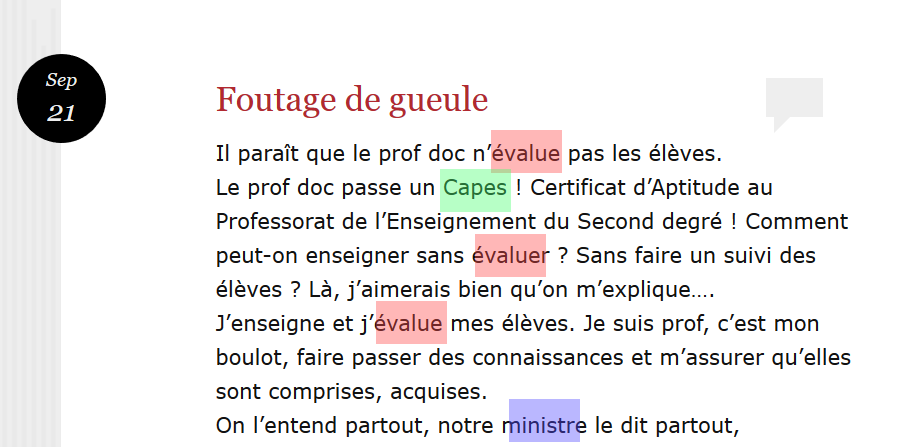
\includegraphics[width=\textwidth]{./Images/blogaladoc2.png}
\end{figure}
\end{column}

\end{columns}

\vspace{0.3cm}

\begin{itemize}
\item chaque \textbf{topic} est une distribution de mots
\pause
\item chaque \textbf{document} est un mélange de quelques topics
\pause
\item chaque \textbf{mot} est tiré au sort dans un topic
\end{itemize}
\end{frame}

\begin{frame}
\begin{tabular}{b{7cm}l}
& \multirow{2}{*}{\includegraphics[scale=0.25]{samm.png}}\\ {\large \textbf{Topic Model (2/2)}}& 
\end{tabular}
\begin{columns}

\begin{column}{0.15\linewidth}
\centering
\begin{figure}

\includegraphics[width=0.7\textwidth]{./Images/topics_inconnus.png}
\end{figure}
\end{column}

\begin{column}{0.65\linewidth}
\centering
\begin{figure}
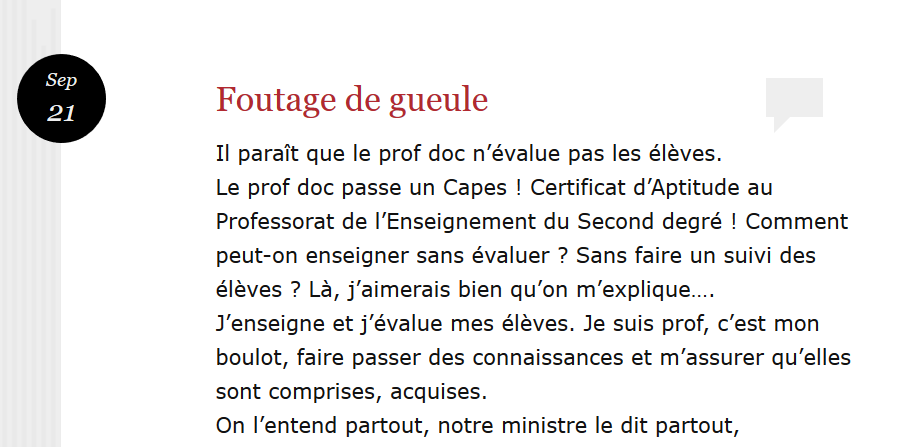
\includegraphics[width=\textwidth]{./Images/blogaladoc.png}
\end{figure}
\end{column}

\end{columns}

\begin{itemize}
\item Dans la réalité, on observe les documents
\pause
\item Tout le reste constitue des \textbf{variables cachées}
\item Nous cherchons à les retrouver, en inversant le processus génératif
\end{itemize}
\end{frame}

\begin{frame}
\begin{tabular}{b{7cm}l}
& \multirow{2}{*}{\includegraphics[scale=0.25]{samm.png}}\\ {\large \textbf{Exemple}}& 
\end{tabular}

\vspace{1.5cm}

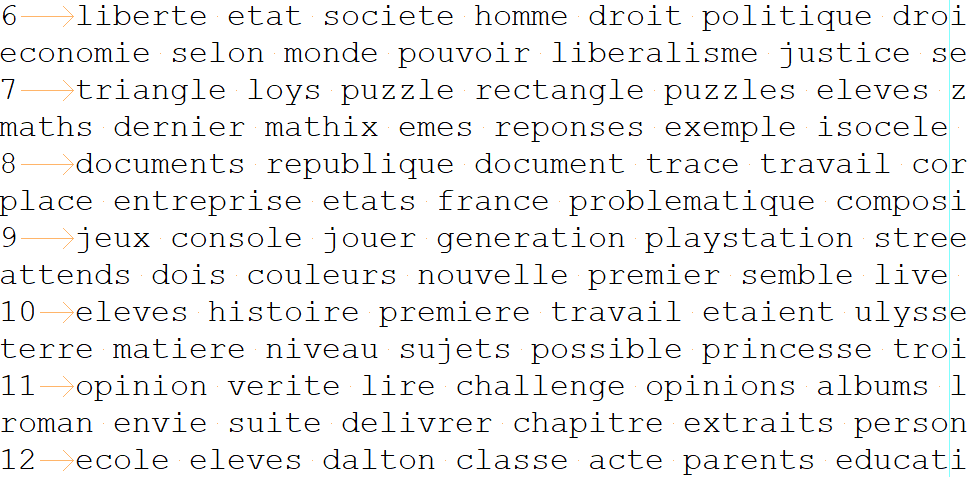
\includegraphics[scale=0.2]{code4-clefs.png}

\end{frame}

\begin{frame}
\begin{tabular}{b{7cm}l}
& \multirow{2}{*}{\includegraphics[scale=0.25]{samm.png}}\\ {\large \textbf{Exemple}}& 
\end{tabular}

\vspace{1.5cm}

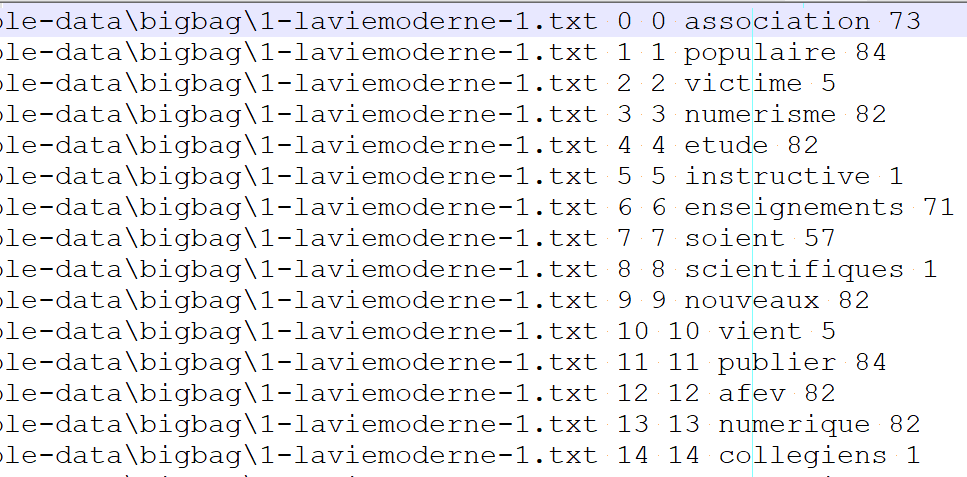
\includegraphics[scale=0.25]{code4-mots.png}

\end{frame}

\begin{frame}

\begin{tabular}{b{7cm}l}
& \multirow{2}{*}{\includegraphics[scale=0.25]{samm.png}}\\ {\large \textbf{Limites et espoirs}}& 
\end{tabular}

\vspace{2cm}


\setlist[itemize]{label=\textbullet}
\begin{itemize}
	\item Hypothèse forte du modèle
	\item Gérer l'hétérogénéité (sur le fond) du corpus
	\item Démarche en échantillonnage/test pour dépasser l'exploratoire.
	\item Vers une constitution itérative du corpus
\end{itemize}



\end{frame}


\end{document}